\chapter{Organization Overview} % Background \& Literature Overview
\label{chap:org}
\textbf{In this section we'll review Tunisie Telecom's History, Notable leaders, Its' business sector and the wide range of clients it offers its services to, as well as its' organizational hierarchy and the work environment I witnessed.  (i.e.\ in the following sections)}
\section{Introduction to Tunisie Telecom \& History} % Some Technique One
\index{Introduction to Tunisie Telecom \& History|(}%%Some Technique One

%\blindtext
\index{Introduction to Tunisie Telecom \& History!Introduction to TT}%%Some Sub-technique One%make it the subsection name
%\blindtext
\subsection{Introduction to TT}%Some Sub-sub-technique One
Tunisie Telecom is the brand name of the historical provider of telecommunication services in Tunisia. Its capital is 875 million euros and its transaction number, in 2004, amounted to 750 million euros.

Tunisie Telecom has more than 6 million fixed and mobile subscribers in Tunisia and abroad. It also plays an important role in improving the Internet's influence in Tunisia, which ultimately allowed it to have 140,000 subscribers by the end of April 2008.
\textbf{Comment: Find more recent data}

\index{Introduction to Tunisie Telecom \& History!History}%%Some Sub-sub-technique One%make it the subsection name to which you want to jump
%\blindtext
\subsection{History}
The law establishing the National Telecommunications Office, whose commercial name is Tunisie Télécom, was promulgated on 17 April 1995 and came into force on 1 January 1996.

Tunisie Télécom sets up, operates and markets the first GSM network in Mauritania (Mattel) from May 2000. It also enters into a technical cooperation agreement with Djibouti Telecom for the development of its telecommunications networks.

It became a public limited company at the end of 2002, it changes its legal status, by a decree of April 5, 2004, to become a limited company called "Tunisie Telecom". It is experiencing partial privatization in July 2006 with the entry into its capital, up to 35\%, of the Emirati consortium EIT (Emirates International Telecommunications).

From 2008, Tunisie Telecom offers the possibility to national bank card holders to feed the balance of their prepaid lines via ATMs of the Arab Tunisian Bank (Mobilink service).

On March 21, 2009, Tunisie Telecom launched a new brand, Elissa, with offers specifically designed for young people under 25; it becomes accessible to all without age limit as of March 10, 2012.

In the spring of 2011, following the Tunisian revolution, the company is shaken by a major social conflict between the representatives of the Tunisian General Labor Union (UGTT) and those of its UAE shareholder over the fate of some 60 contracts representing 3.5\% of the payroll; it is marked by strikes and sit-ins affecting the proper functioning of the operator. It ends with the end of these employment contracts, with the exception of ten contract holders retaining their positions.

In September 2012, Chief Executive Officer (CEO) Ali Ghodhbani retires and is replaced by Mokhtar Mnakri, former CEO of Alcatel's subsidiary.

In 2014, Salah Jarraya was appointed CEO to replace Mnakri, whose term was coming to an end.

In June of the same year, the employees started a social movement to obtain a salary increase and to claim the application of the agreements signed in February 2011. They gather around the UGTT and carry out many work stoppages until May they succeed in May 2015. Following these social movements and strikes, Jarraya resigns on July 2nd.

On August 12, Nizar Bouguila is appointed CEO.

On March 15, 2016, Tunisie Telecom launched its new visual identity called "Life is Emotions", with a new logo. In August, Tunisie Telecom finalizes the purchase of 65.4\% of the entire capital of GO (en).

Bouguila is replaced on September 19, 2017 by Mohamed Fadhel Kraiem. On November 7, Tunisie Telecom signed a five-year contract with the Ministry of Information Technologies and the Digital Economy to cover white areas with broadband telecommunications services.

On December 13, 2017, UAE investment fund Abraaj announced that it had signed an agreement the day before for the definitive purchase of EIT's 35\% stake. However, the bankruptcy of the fund cancels the operation.




%\blindtext

%\blindtext
\index{Introduction to Tunisie Telecom \& History|)}

\section{Global Leaders of Tunisie Telecom}%[Some Technique Two]{Some Technique Two with Super Long Title Which Will Overrun In Header}
\index{Global Leaders of Tunisie Telecom|(}%%Some Technique Two
%\blindtext[5]
Ali Ghodhbani - Mokhtar Mnakri - Salah Jarraya - Nizar Bouguila - Mohamed Fadhel Kraiem

%Imagine some colourful description on Some Technique Three\index{Some Technique Three}.

\index{Some Technique Two|)}

\section{Activities of Tunisie Telecom \& Clients}% Evaluation Criteria
This section should contain information on the metrics and background used to evaluate your work.
\section{Related Work}
\textbf{In this section you need to explain (and reference) similar work in literature}.  Make sure to:

\begin{itemize}
 \item Give a systematic overview of papers with related/similar work
 \item Highlight similarities/differences to your work (perhaps in the form of a table)
\end{itemize}

Note that this section may be sectioned based on the different aspects of your dissertation.  Some referenced text, as an example \citep{Arrighi2003, WithersMartinez2012, Ebejer2016}.

\section{Organizational Hierarchy}
The Organizational Hierarchy of Tunisie Telecom is shown in Figure~\ref{fig:tt1}.
%\begin{figure}[ht!] % supposedly places it here ...
%  \centering
%   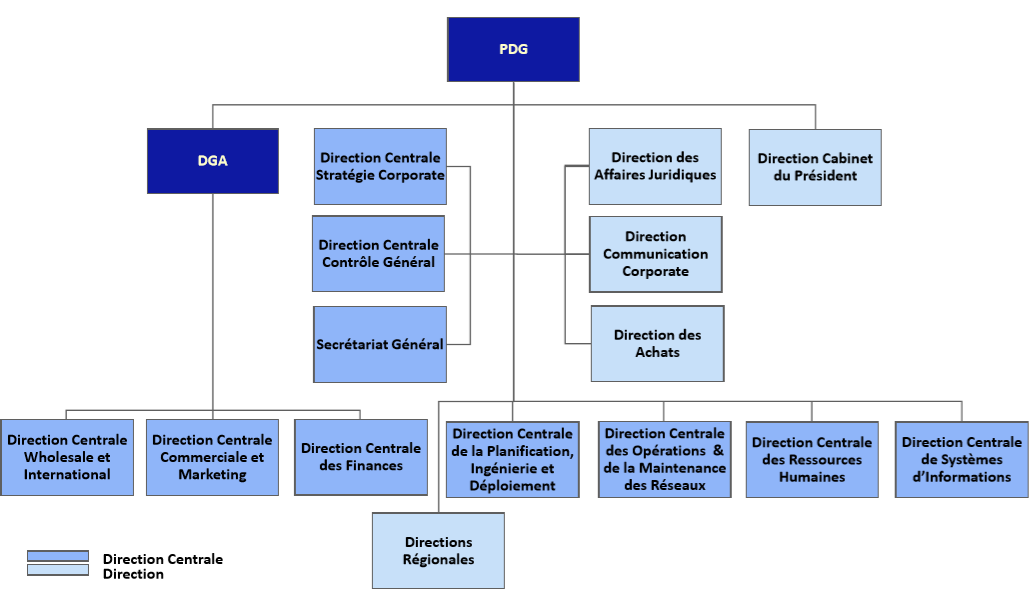
\includegraphics[width=0.6\linewidth]{TT_Hierarchy}
%  \caption[TT Hierarchy]{Tunisie Telecom \index{Goku il-king}}%
%  \label{fig:tt1}
%\end{figure}


% 	To be done later
% ⦁ Structure of the center:

% The belvedere telecommunication complex consists of several centers and services. Following this general presentation, we will move to the precise study of the CC (Switching Center) and the CTN (Digital Transmission Center) where we spent the month of internship.

% Figure 3: Center Structure
% ⦁ Line switching center:

% The CCL is a service that manages the maintenance of the switched network and the installation of transmission cables that connect the subscribers to the central office and the exchanges between them.
% ⦁ Switching Center:

% The Belvedere complex contains two switching exchanges intended to maintain the switching system; The ERICSSON Swedish AX system and the German EWSD system from Siemens. The center is responsible for all subscriber registration operations in the system as well as operations related to fixed telephony services such as prepaid, international calls or caller ID display.
% ⦁ Digital Transmission Center:

% The digital transmission center is one of the basic cells in the telecommunication network. It is the speaker of digital transmission media. In a future chapter of our report, we will take care of his presentation.



% 	This is an Image outlining the Organizational Hierarchy of Tunisie Telecom



\section{Work Environment}
\blindtext